\section{Trabajo Adelantado}\label{sec:tra}


\subsection{Exploración a través de Focus Groups}
    \par Una de las problemáticas del trabajo realizado, era validar con usuarios del \acrshort{dcc} las propuestas obtenidas de la investigación teórica. A modo de recoger sus preferencias de manera explícita en la interacción con el sistema. Para esto, se llevaron a cabo dos \textit{\acrlong{fg}}. En ellos se realizaron consultas en torno a la información a la que se puede acceder a través del bot, información sugerida a través del comportamiento social, el tutelaje, la motivación para obviar el contacto directo con personas, privacidad y opciones de notificación.
    
    \subsubsection{Caracterización de los participantes}
    \par Los participantes del primer \acrshort{fg}, son alumnos y ex-alumnos del \acrshort{dcc}. De estos, ocho de los nueve han presentado problemas relativos a información académica, es decir, la falta de información o información errónea les ha dificultado el avance en algunos procesos académicos. Cinco de nueve no han cursado ningún ramo relativo a la memoria, sin embargo todos han participado de procesos con plazos como las prácticas profesionales o \acrlong{ps}. En el caso del segundo \textit{\acrlong{fg}} las características son similares, pero son solo cuatro alumnos
    
    \subsubsection{Respuestas de los estudiantes}
    \par A continuación se detallan los resultados obtenidos para las categorías anteriormente descritas. Los resultados mostrados responden a análisis en conjunto de ambos \textit{\acrlong{fg}}, por lo tanto de aquí en adelante cuando refiramos este término nos estaremos refiriendo al proceso de consulta completo.
    
    \begin{itemize}
    \item \textbf{Información a la que se puede acceder a través del bot:} El contenido al que se puede acceder actualmente a través del bot, son solamente las preguntas frecuentes. En relación con las nuevas funcionalidades de suscripción se les preguntó a los estudiantes cuál era la información relevante para ellos, sobre qué cosas querían un recordatorio o sugerencias.
    \par La mayoría está de acuerdo en que las fechas, ya sean de apertura o cierre de procesos, incluso tareas o avances parciales serían un contenido que ellos desearían del bot, cómo una notificación. También los cambios en la información relativa a un proceso, se deberían comunicar oportunamente, por otro lado, no se debería notificar un cambio de plazo, sino ajustar los recordatorios a los nuevos plazos. Cómo sugerencias, se admiten temas relacionados con los procesos en los que se esté suscrito o se haya preguntado reiteradamente ya sea por parte del usuario o por usuarios "similares".
    \par Aparte de las notificaciones, se sugirió dar acceso a información relevante del proceso en cuestión, como el contacto público de personas relacionadas con el proceso (correo el coordinador del \acrshort{e}, contacto de la secretaria docente, por decir algunos) y ejemplos de válidos de los requisitos para cierta etapa (preinscripciones de práctica, ejemplos de propuestas de memoria).
    \item \textbf{Información Social: } Sobre este punto la consulta venía en torno a si estarían dispuestos a recibir sugerencias a partir de otros usuarios con perfiles similares.
    Aquí las opiniones estaban divididas. Aunque en el alumnado se es reticente a compartir información con terceros, no habría problemas en que fuera información exclusivamente académica, relacionada con fines laborales o información que otros organismos ya tengan.
    \item \textbf{Tutelaje:} La idea de esta pregunta era saber qué tan dispuestos están en involucrar un tercer actor que pueda ayudar en un proceso académico, al que denominaremos tutor, por ejemplo que el profesor guía recibiera un aviso cuando el alumno no respondiera ni interactuara con el bot durante el proceso de titulación. Las respuestas dan cuenta de que no hay un acuerdo claro en cuanto a esto. Para algunos era algo viable, para otros era algo opcional, mientras que unos pocos preferían descartar de plano.
    \par Finalmente a pesar de los cuestionamientos a su funcionalidad y a la forma de usar los bots de cada alumno. Se pudo consensuar que: Fuera una opción habilitada por el usuario y con posibilidad de deshabilitar en cualquier momento, coloquialmente "cómo hacer un sudo". Así mismo, los parámetros asociados a este tercero como el contacto e información a la que accede también deberían ser definidos por el usuario. De esta forma, elegir al "tutor" que cada usuario decida y asociado al aspecto que él decida.
    \item \textbf{Motivación para obviar el contacto:} Esta pregunta busca profundizar en las razones de por qué los alumnos podrían preferir el bot al contacto directo con otra persona. En este caso, las razones son diferentes para cada alumno, pero concuerdan con la literatura de lo que se busca en un sistema de información \cite{Thurman}. Algunas de ellas son ansiedad producto de la interacción, para no molestar, porque las preguntas son repetitivas y algunas mejoras funcionales como la rapidez, sugerencias a temas que tal vez no surjan de una pregunta directa a un encargado humano, la libertad de acudir cuando se desee y la sensación de control sobre la interacción.
    \item \textbf{Privacidad:} Dentro de este ítem, se preguntó específicamente por la privacidad de la información que el bot pudiera almacenar, y que \textit{trade-off} estarían dispuestos a realizar por más funcionalidades. Aquí hay acuerdo en que debería ser la mínima posible y en caso de ser más solo información académica. Por otro lado, la mayoría estuvo de acuerdo en conceder permisos temporales y sin guardar información de forma permanente, en caso de que alguna funcionalidad requiera más información. De este modo se vuelve a repetir la configuración y permisos personalizados a cada alumno.
    
    \item \textbf{Opciones de notificación:} En el caso de las opciones de notificación se puede observar se puede observar que las notificaciones deberían ser en general cortas con poca información y que también fueran personalizables. Cada notificación debería mostrar el área a la que pertenece o una forma de saber qué temática o relacionado con qué es esa notificación. Al mismo tiempo, debería ser capaz de explicar en breves líneas que es la información nueva y en el caso de requerir más espacio, texto o se necesite mostrar más contenido debería agregarse un link o un enlace en el que se pueda desplegar a través de una página o un blog la información necesaria pero no directamente en el Chat.
    \end{itemize}
    \subsubsection{Análisis y conclusiones}
    \par A pesar de que en el \textit{focus group} se puede ver una ligera tendencia a ciertas características a partir del grado de avance de los alumnos, en general lo que se puede observar es que no hay una correlación directa entre el grado de avance y las preferencias personales de cada alumno, así que se propone una caracterización alternativa, asociar a los estudiantes en tres grupos: Aquellos que prefieren definir absolutamente todos los parámetros de su interacción, otros que prefieren que se les sugiera o lo que se les facilite la interacción, mientras que los terceros serían algo así como un usuario mixto que prefiere cierto grado de personalización mientras que prefiere una simplificación de otras tareas.
    \par Generalmente los alumnos que prefieren una alta especificación o definir cada una de las características, están también ligados a un alto grado de valoración de la privacidad y configuración manual. Se perciben a ellos mismos como autosuficientes,
    \par Por otro lado, los alumnos que suelen tener un interés más práctico, valoran entablar la menor cantidad de interacciones posibles y valoran mucho más la eficiencia del flujo de trabajo y su tiempo. Generalmente se perciben a sí mismos como no tan atentos a las tareas y algo desconcentrados.
    \par A partir de esto vamos a caracterizar los tres grupos de estudiantes con tres nombres el primero sería un \acrfull{S}, el segundo vendría ser un \acrfull{R} y el tercero vendría ser un \acrfull{P}.
    \par También podemos caracterizar la forma en que persiguen sus objetivos, los distintos actores en el sistema, esta puede variar dependiendo del proceso en el que se esté, la experiencia previa y las preferencias personales. Cabe destacar que no responden específicamente las caracterizaciones de cada uno de los alumnos es decir un \acrshort{P} aun así puede querer valorar o perseguir la privacidad al consultar información y también un \acrshort{S} puede perseguir la funcionalidad de los recordatorios.
    \begin{figure}[h]
        \centering
        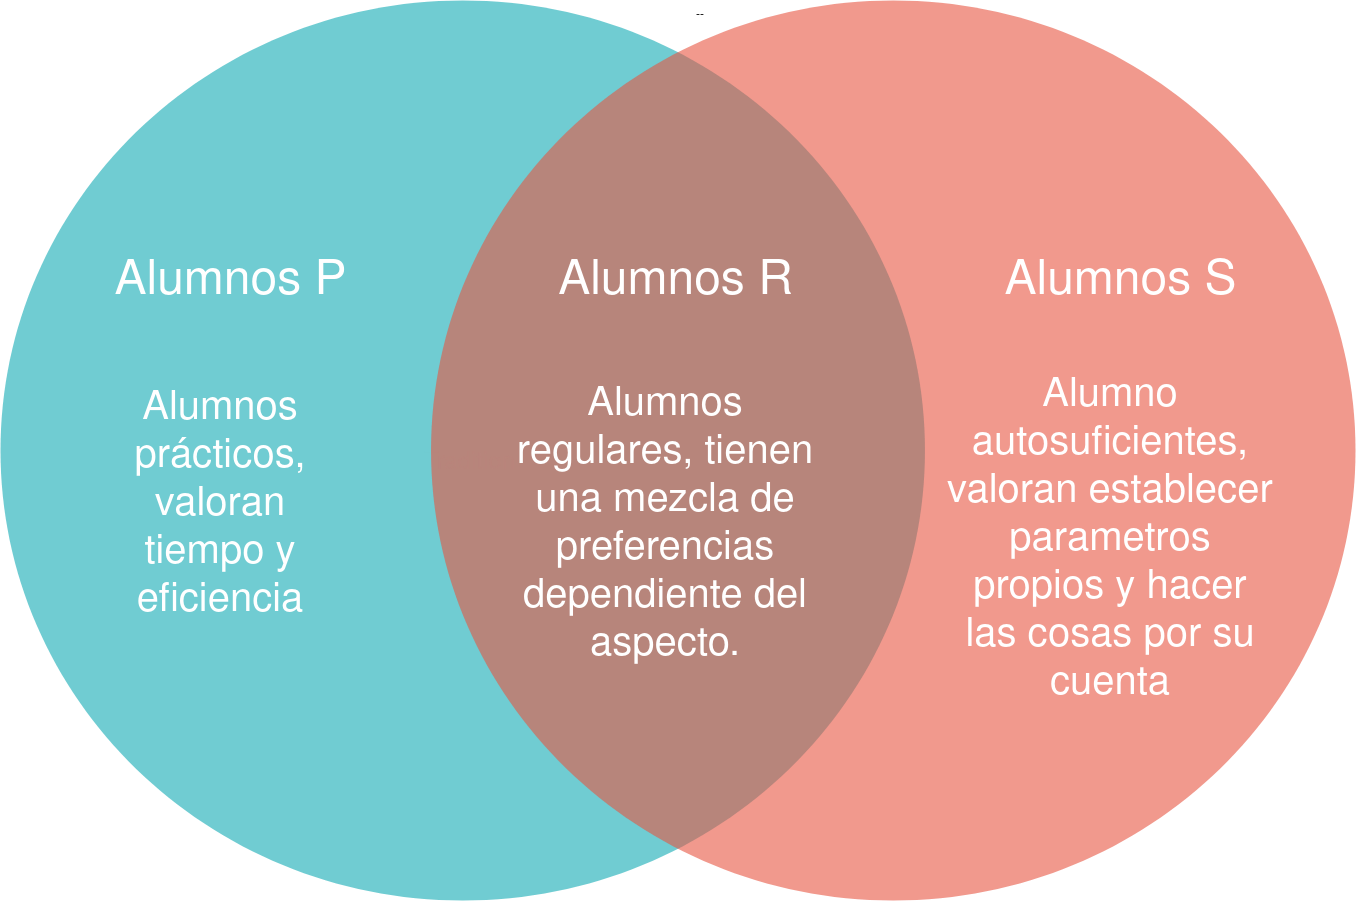
\includegraphics[scale=0.2]{02-informe/imagenes/focus_groups/Tipos_de_alumnos-Diagrama_de_Venn.png}
        \caption{Diagrama de Venn: que representa los tipos de estudiantes encontrados en el \textit{Focus Group}.}
        \label{fig:alumnosVenn}
    \end{figure}
    \par Como conclusión se puede ver una tendencia a la personalización de la mayoría de los elementos funcionales, a sí mismo el contenido. En el caso de la privacidad, se debería poder elegir tanto que permisos son dados así como su duración, en el caso de las notificaciones poder establecer su frecuencia en cualquier momento, en el caso de las sugerencias se accede a entregar más información o recibir sugerencias siempre y cuando esto sea establecido por el usuario y que la información dad tenga el carácter de input temporal y no almacenado. Así mismo se establece que el tutelaje debe ser definido por el usuario. Todo esto va en línea con la investigación preliminar que sugiere que los usuarios valoran la personalización y lo relevante de la información para cada usuario suele ser completamente diferente. Todo lo anterior, hace que este trabajo esté orientado en la dirección de las necesidades y preferencias del estudiantado, al mismo tiempo que va en línea con los descubrimientos y los trabajos relacionados.

\subsection{Nuevos Modelos de Interacción}
    \par En esta sección se detalla las problemáticas de diseño de los nuevos modelos, luego se condensan los tipos de contenido que debería tener el sistema, las funcionalidades y las modalidades de interacción que surgen de las preferencias de los usuarios
    \subsubsection{Problemáticas de diseño de los nuevos modelos}
    \par A partir de la diversidad de opinión y de preferencia que se extrae de la investigación a través de \acrshort{fg}, podemos ver que la complejidad del modelo subyacente a tales impresiones es alta. Por la misma razón, el sistema va a tener una manera diferente de concretar los objetivos de estos actores dependiendo de cuáles sean estos objetivos y cuáles sean las tareas o requisitos asociados a tales objetivos. A raíz de esto, se hace extremadamente necesario poder especificar con claridad cada uno de los requisitos y sin embargo poder englobarse en funcionalidades que respondan de manera unilateral a las necesidades de las personas, es decir a través de la misma interfaz, la del chatbot. Por eso es que antes de involucrarnos en el diseño funcional o computacional o generar algún diagrama como el de arquitectura o de clases. Se hace necesario plasmar de manera clara las diferentes necesidades de los alumnos en el sistema, las características de estos objetivos, sus relaciones y como pueden ser llevados a la concreción.
    
    \par Estas diferencias de parecer y de uso, hacen que el sistema a crear deba ser altamente configurable, es decir que cada usuario puede definir que quiere y cómo lo quiere. El cómo responder a las necesidades de los distintos usuarios determina las funcionalidades del sistema, así mismo el qué o la propia necesidad por un contenido específico determina cuál será la información del sistema. A partir de esto, podemos resumir lo que buscan los diferentes usuarios en el sistema en dos grandes categorías contenido, es decir fechas, definiciones, actores relacionados, requisitos, consecuencias, etc. y funcionalidades, tales como recordatorios, consultas, entre otros.
    \par Desde esta separación preliminar se proponen diferentes definiciones y diagramas, los que ayudan a encapsular y explicar de manera concisa y clara el modelo de interacción de alumnos y alumnas, sin perder el foco en los objetivos de los mismos.
    \par Para lograr esto se propone la adopción de la simbología del lenguaje gráfico \gls{i*} \cite{Dalpiaz2016}, con el fin expresar de forma correcta a los actores involucrados, sus preferencias y asimismo las tareas subyacentes que el sistema debería realizar para completar los objetivos que cada uno de estos actores tiene.
    \par A partir de la investigación del estado del arte, la exploración a través de \textit{focus groups} y el análisis posterior, se define lo siguiente:
    
    \subsubsection{Contenidos del Sistema}
    \label{sssec:contenidos}
    \par Los contenidos que buscan los alumnos a través del bot los podemos agrupar en cuatro categorías Definiciones, Requisitos, Fechas y Actores.
    \par las Definiciones son la descripción o detalle del proceso, a grandes rasgos, es una explicación de se trata el proceso, como su nombre lo expresa muy bien, cumplen un rol \textit{educativo}, que es informar al usuario de que es lo que se trata este proceso. La idea de este tipo de información es que el usuario puede entender en una sola consulta que es el proceso, de que trata, que consigue con él, de forma eficiente y amigable.
    \par Los Requisitos son todas aquellas cosas que serán solicitadas durante el proceso, y que permiten el avance durante el mismo. El alumno busca enterarse de cuáles son estas cosas, que tareas o asignaciones debe realizar para lograrlo y ejemplos válidos de una tarea completada. Por ejemplo, un ejemplo de requisito para el proceso de práctica sería realizar la preinscripción de práctica. Al consultar en el sistema el alumno debería obtener el requisito junto a una explicación de en qué consiste y un ejemplo válido de cómo realizarla.
    \par Las fechas son todas aquellas fecha relevantes en un proceso, en general definen plazos o hitos durante el proceso. Por ejemplo la fecha de entrega del primer avance en el \acrshort{e}
    \par Los actores son todos aquellos entes relacionados con un proceso, tienen cuatro características que serían: el rol que cumplen dentro del proceso (el cargo o responsabilidad dentro del proceso), el contacto (medio para localizarlos), proveen de un servicio dentro del proceso (las tareas asignadas a su rol) y tendrían una asociación o un grupo al que pertenecen, por ejemplo dentro de una categoría "tipo profesor" este podría pertenece al rol de "Académicos" o "Universidad", mientras que una institución que provee de prácticas podría pertenecer a la categoría de "Externos" o "Lugares de práctica".
    \subsubsection{Funcionalidades relativas a la información}
    \par Las funcionalidades buscadas se puede agrupar también en 4 grupos: Consultas, Sugerencias, Intervenciones y Recordatorios.
    \par Las Consultas son un tipo de interacción ya presente y que consiste en acceder al bot para realizar alguna consulta sobre la información de un determinado proceso, esta información podría ser cualquiera de los contenidos listados arriba.
    \par Las Sugerencias son de un formato similar a las consultas, pero son entregadas sin ser solicitadas directamente, debe poder activarse y desactivarse, además de que no deben ser entregadas en cualquier momento, sino ojalá con una periodicidad predeterminada por el usuario, buscan ayudar al usuario a encontrar o enterarse de contenido que podría serle de utilidad sin ser buscado directamente, es decir a partir de su interacción y usuarios con características similares.
    \par Los recordatorios son un tipo especial de notificación que es gatillada expresamente por el usuario quien les fija una periodicidad o frecuencia, buscan ayudarlo a programar y efectuar los trabajos de manera efectiva. Tienen la opción de requerir feedback si el usuario así lo desea, para motivar el compromiso.
    \par Las intervenciones son habilitadas por el usuario y permiten al bot enviar notificaciones que alteren o podrían alterar el curso conocido del proceso, estas notificaciones pueden ser enviadas tanto al estudiante cómo al estudiante, cómo a un tercero que estudiante defina, en variados casos. Por ejemplos, los cambios en los requisitos serían una intervención, y esa modificación sería enviada al alumno. Por otro lado un cambio de fechas no siempre se categorizan como intervención, dependiendo del alumno, y del plazo. Por esta razón las intervenciones tienen un periodo de vigencia, en el que son relevantes y deberían proveer idealmente suficiente marco de acción para tomar medidas pertinentes al caso. También podrían ser provocadas por el estudiante al no responder a una interacción pactada como los recordatorios, siempre y cuando esto haya sido habilitado y parametrizado por el alumno.
    
    \subsubsection{Modalidades de Interacción}
    \label{sssec:cualidades}
    \par la mayoría de reticencias o preferencias de los alumnos, respecto a como se deben llevar a cabo las tareas asociadas a los objetivos de contenido o funcionalidad, se pueden agrupar en 5 categorías Privacidad, Parametrización, Eficiencia, Individualidad y Confiabilidad.
    \par la Privacidad hace referencia a la información que el alumno debe entregar para obtener cierta funcionalidad o contenido. En general se busca que exista la mayor privacidad posible, pero algunas interacciones contienen un \textit{trade-off} entre privacidad y eficiencia por ejemplo, que algunos alumnos están dispuestos a aceptar.
    \par La Parametrización tiene que ver con la configurabilidad de la funcionalidad en cuestión, dependiendo del estudiante es más o menos valorada, y esto implica que el sistema debe dar las opciones de parametrización al tiempo que simplificarlas dependiendo del alumno.
    \par La Eficiencia hace referencia a que tan bien puedo cumplir la tarea en cuestión, usualmente relacionada a obtener más recursos o simplificar las parametrizaciones de una funcionalidad determinada.
    \par La Individualidad propone la autonomía del usuario en esa funcionalidad, por ejemplo, buscar contenido de memoria o de práctica sin avisar a otros actores. O no avisar inmediatamente al profesor guía de una omisión sin que el alumno haya consentido esto.
    \par La Confiabilidad por último hace referencia tanto a la validez de la interacción como la confianza que alumno puede descargar en tal interacción. Por ejemplo, que los contactos consultados de un determinado actor estén vigentes.
    
    \subsubsection{Resumen conceptual del modelo de Interacción}
    \par este resumen pretende expresar de manera breve, los diferentes contenidos, funcionalidades y modalidades a través de un diagrama jerárquico de clases o de conjuntos. Cómo se podrá observar más tarde en la sección \ref{sssec:diagramas}, las funcionalidades determinan de qué forma se quiere obtener un determinado recurso del sistema, son la interfaz funcional del sistema. Por otro lado los contenidos, son los datos que el sistema debe almacenar para posteriormente servir, estos a su vez definen modelos de datos de la información del sistema. Finalmente las Modalidades hacen eco de los valores presentados en la interacción alumno-bot.
    
    \begin{figure}[h!]
        \centering
        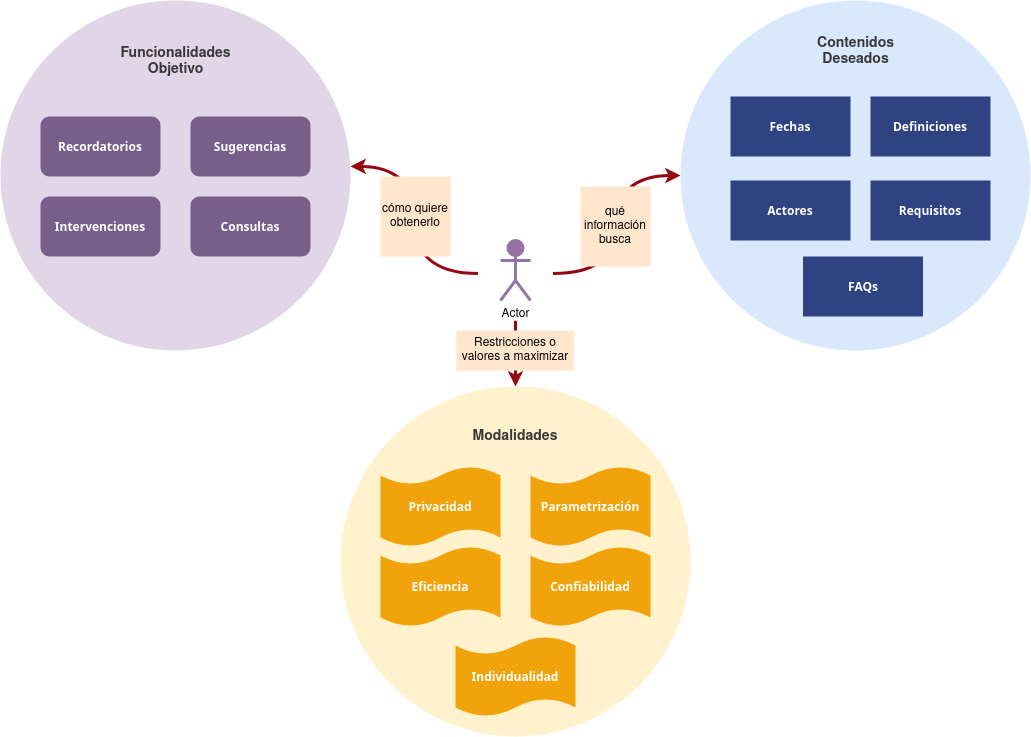
\includegraphics[scale=0.4]{02-informe/imagenes/modelos_de_interacción/objetivos_y_cualidades.png}
        \caption{Diagrama que busca plasmar las superclases en las que se agrupan los objetivos de los alumnos a sí como las funcionalidades del sistema. Todo agrupado en categorías}
        \label{fig:my_label}
    \end{figure}
    
    \subsubsection{Notación i*}
    \par La notación \gls{i*}, se usará como se explicó anteriormente para explicar no solo la interacción del usuario con el sistema, sino también que persiguen los mismos al realizar dicha interacción.
    \par Las bases del lenguaje se pueden encontrar en la guía del lenguaje \cite{Dalpiaz2016} y las imágenes en la wiki del lenguaje \cite{No-mention2011}.
    \par esto se hace a través de la sintaxis de este lenguaje que detallaremos brevemente a continuación:
    \begin{itemize}
        \item Objetivos: los objetivos o \textit{Goals} por su nombre en inglés, son en palabras simples un estado que desea alcanzar el usuario relativo a algo. Por ejemplo: `` Tener los pasajes de avión comprados``
        \begin{figure}[h]
            \centering
            
\includegraphics{02-informe/imagenes/i_star/goal.jpg}
            \caption{Objetivo \gls{i*}}
            \label{fig:my_label}
        \end{figure}
        \item Tareas: las tareas (\textit{Task}) son acciones que el usuario puede realizar para lograr su objetivo. Ejemplo: ``Buscar pasajes de avión``, `` Comprar pasajes en la aerolínea``.
                \begin{figure}[h]
            \centering
            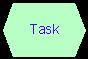
\includegraphics{02-informe/imagenes/i_star/task.jpg}
            \caption{Tarea \gls{i*}}
            \label{fig:my_label}
        \end{figure}
        \item Cualidades: o \textit{Qualities} son maneras o elementos de valor que se quiere preservar u obviar al completar un objetivo. Ejemplo: ``Rápido``, en esta serie de ejemplo la frase completa se entendería como ``Tener los pasajes de avión comprados rápido`` o de manera ``rápida``.
                \begin{figure}[h]
            \centering
            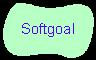
\includegraphics{02-informe/imagenes/i_star/softgoal.jpg}
            \caption{Cualidad \gls{i*}, antes \textit{softgoal} en i* 1.0}
            \label{fig:my_label}
        \end{figure}
        \item Recursos: Los recursos son elementos ligados a las tareas, como una ``tarjeta de crédito``, en esa línea se podría ``comprar los pases en la aerolínea con una tarjeta de crédito``
                \begin{figure}[h]
            \centering
            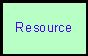
\includegraphics{02-informe/imagenes/i_star/resource.jpg}
            \caption{Recurso \gls{i*}}
            \label{fig:my_label}
        \end{figure}
        
        \item Actores: Los actores son elementos principales del diagrama, realiza acciones, dispone los recursos y tiene objetivos. Pueden ser de tres tipos: un tipo general del cuando no se desea especificar, un agente que representa una instancia particular de un actor: como ``Juan`` o el ``Bot`` y un rol, que viene a ser una categoría o clase como ``Estudiante``. Las \textit{boundaries} o límites relativos a un actor determinan que elementos le ``pertenecen``
        \begin{figure}[h!]
            \centering
            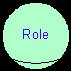
\includegraphics[scale=0.4]{02-informe/imagenes/i_star/role.jpg}
            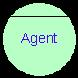
\includegraphics[scale=0.4]{02-informe/imagenes/i_star/agent.jpg}
            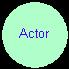
\includegraphics[scale=0.4]{02-informe/imagenes/i_star/actor.jpg}
            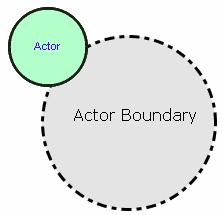
\includegraphics[scale=0.4]{02-informe/imagenes/i_star/actorboundary.jpg}
            \caption{Actores \gls{i*}}
            \label{fig:my_label}
        \end{figure}
        \item Enlaces: o \textit{Links} son lo que representa las relaciones entre los diferentes elementos del sistema, pueden representar dependencias, contribuciones, especificaciones o incluso notar una contribución. En el caso de este trabajo se usan principalmente 3 tipos de enlaces:
        \begin{itemize}
            \item Dependencias: Se indican con una letra D y expresan que el elemento a la izquierda de la dependencia, depende del elemento a la derecha, de manera un poco simplista.
            \begin{figure}[h!]
                \centering
                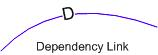
\includegraphics[scale=0.6]{02-informe/imagenes/i_star/dependencylink.jpg}
                \caption{Dependencia \gls{i*}}
                \label{fig:my_label}
            \end{figure}
            \item Contribuciones: Indican que cierto elemento contribuye a una Cualidad, puede ser de 4 formas, satisfaciendo completamente lo que se nota con \textit{make} sobre el enlace, Imposibilitando su realización lo que se denota con \textit{break}, o ayudando un poco o debilitando un poco lo que se denota con \textit{help} y \textit{hurt} respectivamente.
            \begin{figure}[h!]
                \centering
                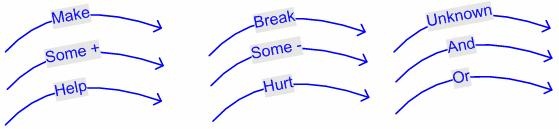
\includegraphics[scale=0.6]{02-informe/imagenes/i_star/contribuitonlinks.jpg}
                \caption{Contribuciones \gls{i*}}
                \label{fig:my_label}
            \end{figure}
            \item Refinamiento: Expresan que un objetivo o tarea tiene otros elementos que lo definen. Pueden ser O (\textit{OR}) o Y (\textit{AND}), lo que determinan es que para que el objetivo se satisfaga se debe satisfacer a su vez todos los elementos que lo refinan (\textit{AND}) o alguno de ellos (\textit{OR}).
            \begin{figure}[h!]
                \centering
                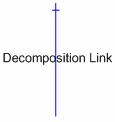
\includegraphics[scale=0.6]{02-informe/imagenes/i_star/decomposition.jpg}
                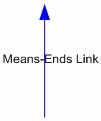
\includegraphics[scale=0.6]{02-informe/imagenes/i_star/meansendslink.jpg}
                \caption{Refinamiento \gls{i*}}
                \label{fig:my_label}
            \end{figure}
                    
        \end{itemize}
    \end{itemize}
    
    \newpage
    \subsubsection{Diagramas de Funcionalidades y Objetivos}
    \label{sssec:diagramas}
    
    \par A continuación se modelará la interacción de un usuario con el proceso de titulación a través del lenguaje \gls{i*}. En cada uno de los diagramas siguientes, se expresan las funcionalidades a las que el alumno podrá acceder en el sistema, en ellos se podrá ver cómo es que ciertas funcionalidades tienen que buscar un equilibrio entre las distintas cualidades o modalidades preferidas por el alumno.
    \par Los diagramas se explican uno por página, esto se hace con el objetivo de que el análisis de cada uno quede exactamente bajo la imagen.
    
    \newpage
    \par \textbf{Consultas}
    \begin{figure}[h!]
        \centering
        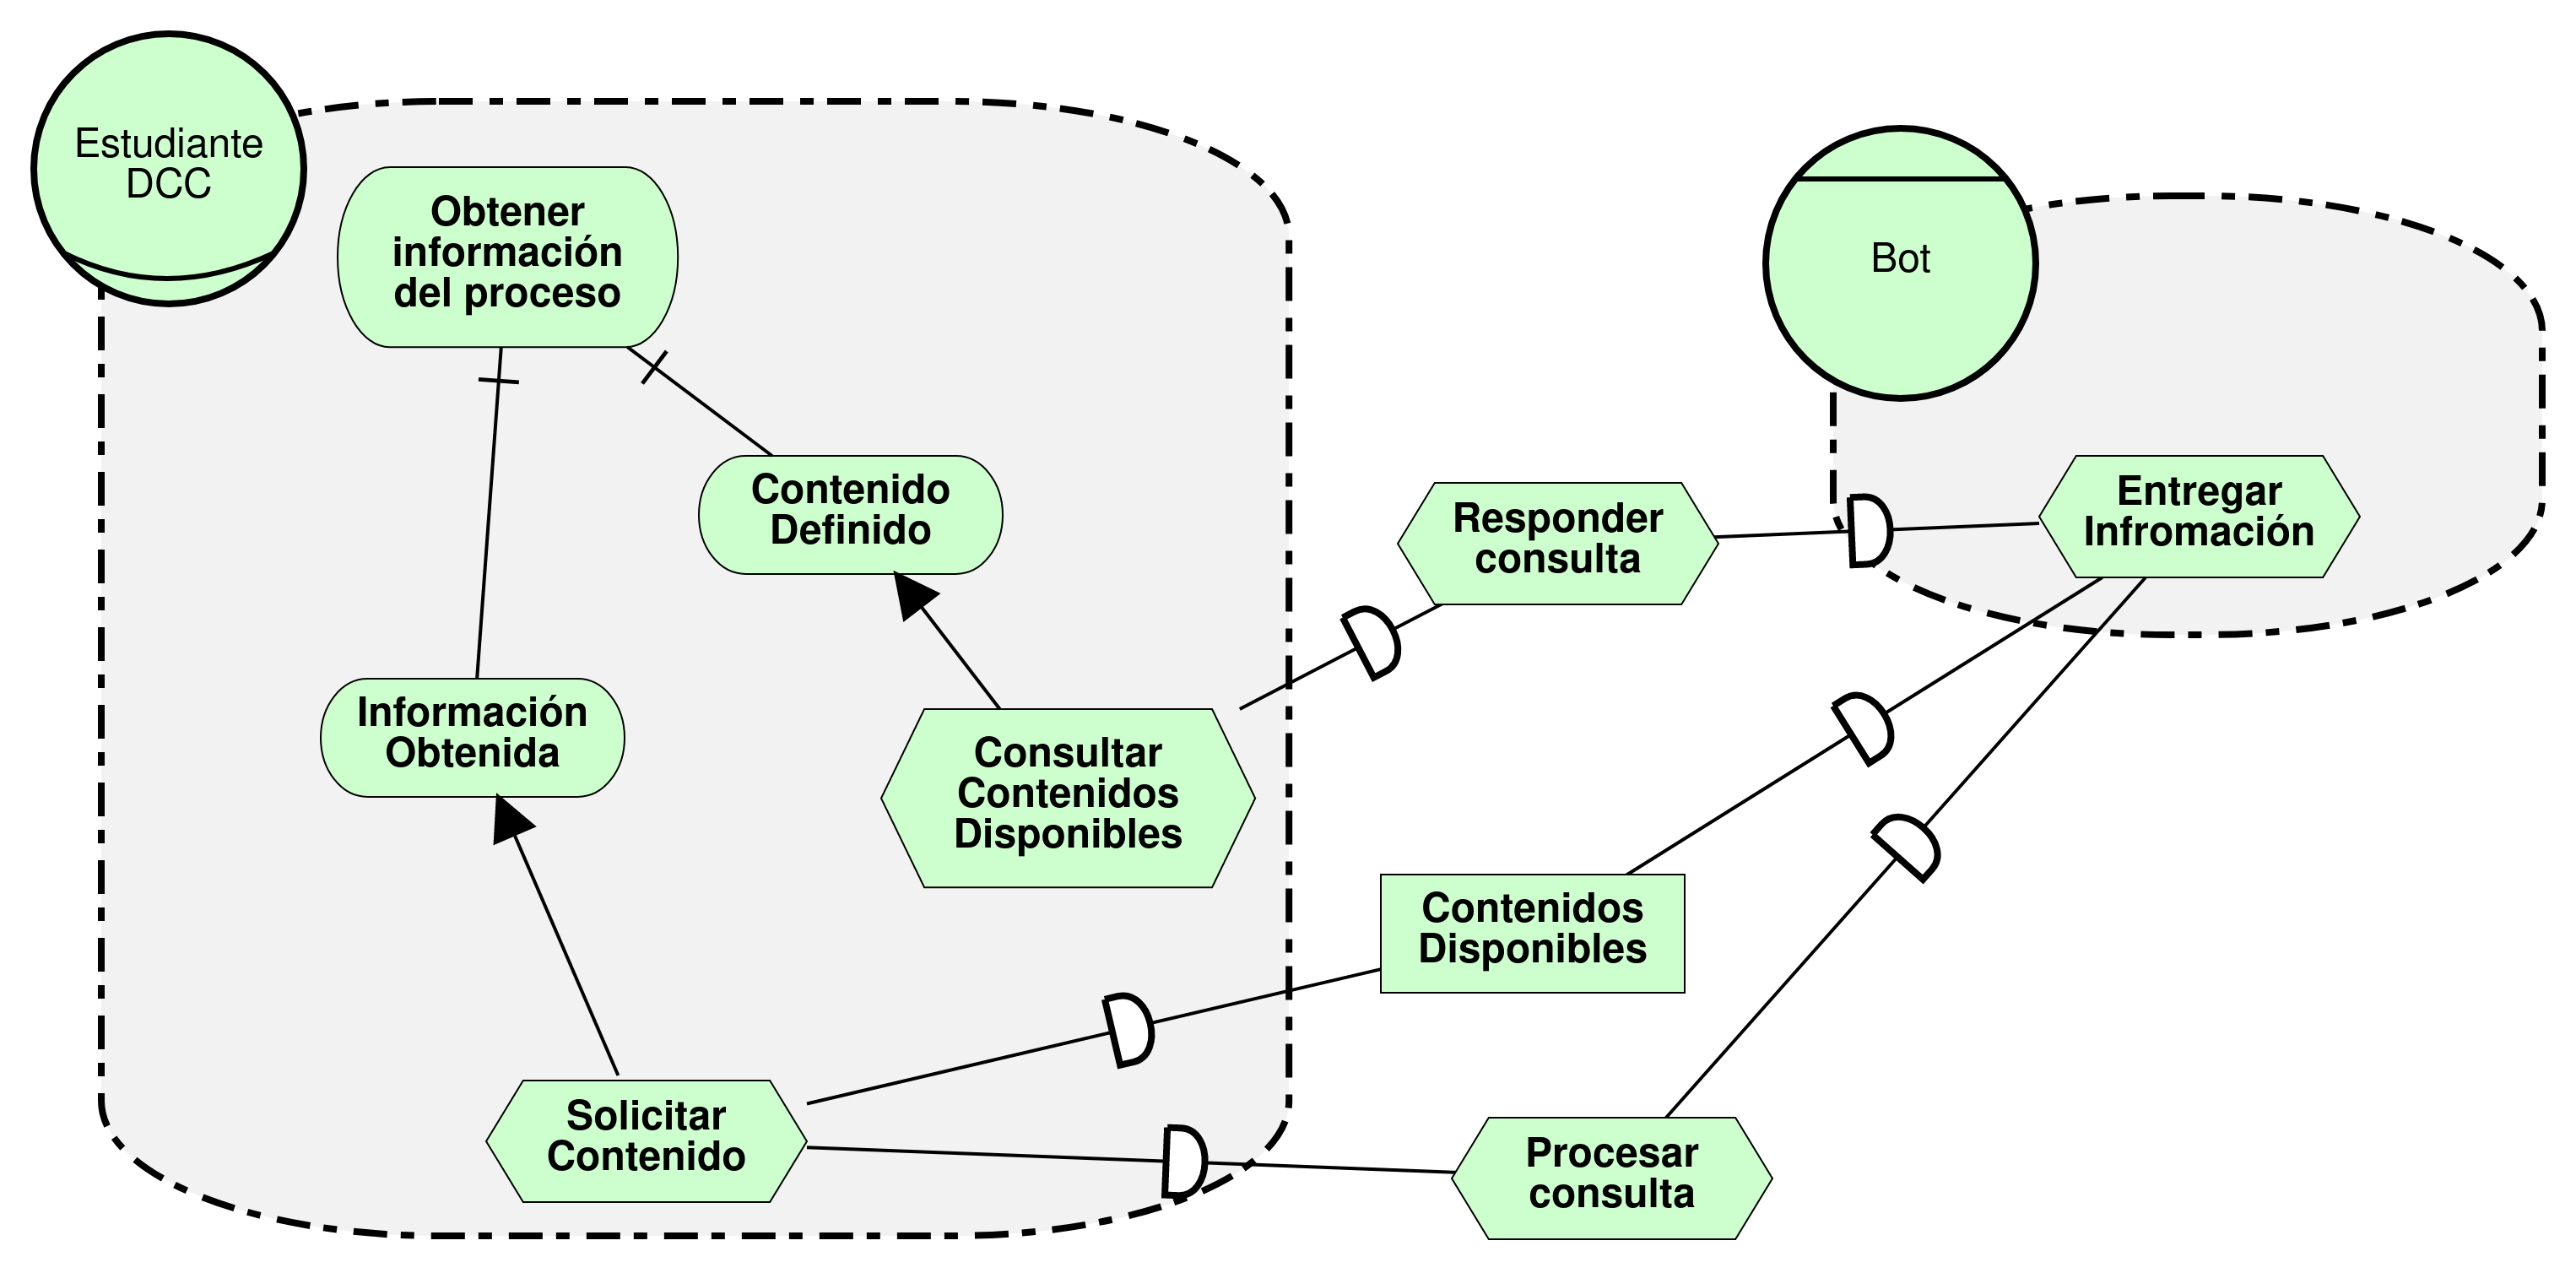
\includegraphics[width=\textwidth]{02-informe/imagenes/modelos_de_interacción/Consultas.png}
        \caption{Modelo de Interacción de consultas sobre contenido de un proceso al bot. En sintaxis i* 2.0}
        \label{fig:consultas}
    \end{figure}
     
     \par Las Consultas, son la interacción básica del bot, de hecho ya están implementadas de alguna manera con las preguntas frecuentes. En este proceso cómo se puede ver en la figura \ref{fig:consultas}, solo se solicita algún contenido relativo a un proceso y es entregado de vuelta. Se debe tener en cuenta que ahora, este contenido es cualquiera de los listados en \ref{sssec:contenidos} \nameref{sssec:contenidos}, por ende la consulta sólo podrá ser contestada con la información que se encuentre disponible.
     \par A pesar de que no se muestra en el diagrama, podría ser factible agregar el modelo del asistente de las FAQs, esto aún está bajo evaluación.
     Cómo se puede observar en la \ref{fig:consultas}, el proceso de realización de consultas no está asociado de forma relevante con ninguna de los temas más controvertidos del bot, y por ende no se detallan cualidades en este diagrama.
     
     \newpage
     \par \textbf{Recordatorios}
    \begin{figure}[h!]
        \centering
        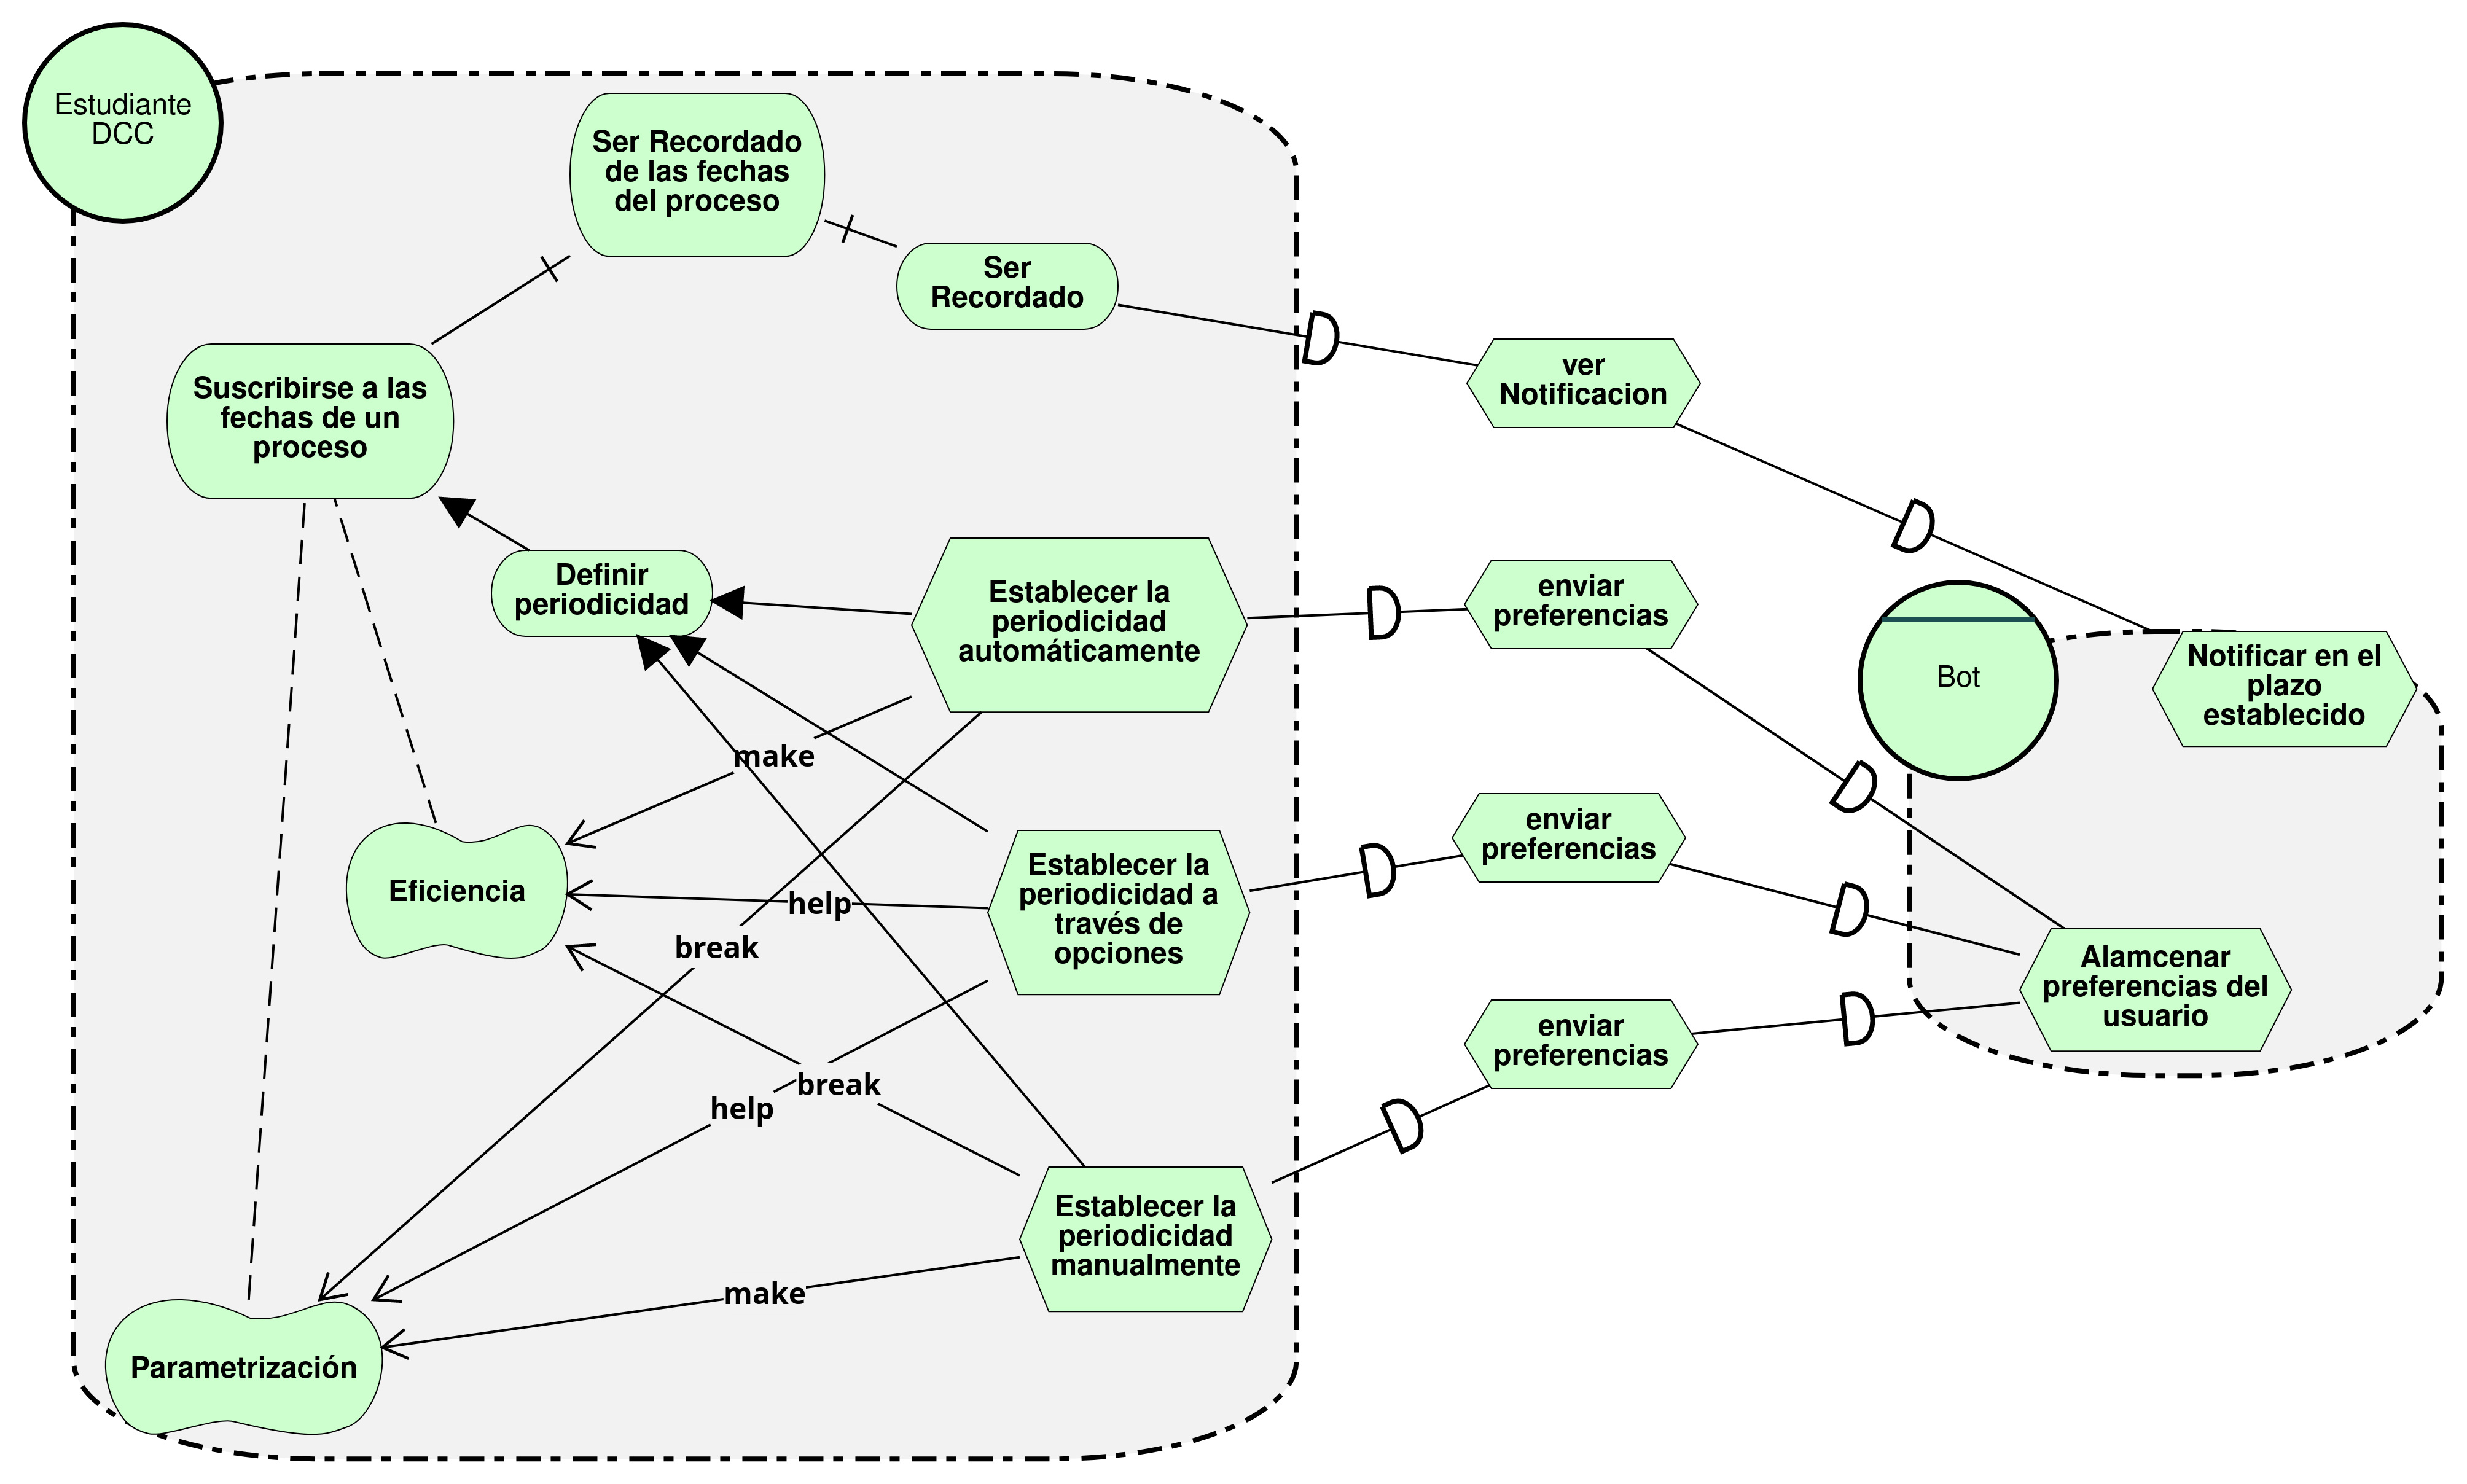
\includegraphics[width=\textwidth]{02-informe/imagenes/modelos_de_interacción/Recordatorios.png}
        \caption{Modelo de Interacción para la suscripción a los recordatorios de un proceso a través bot. En sintaxis i* 2.0}
        \label{fig:recordatorios}
    \end{figure}

    \par Los recordatorios son una de las funcionalidades que mejor acogida tuvo durante el proceso de investigación con alumnos. Sin embargo, para recoger las preferencias de todos los grupos, se hace patente que hay que hacer una elección entre las cualidades de Eficiencia y Parametrización detalladas en \ref{sssec:cualidades} \nameref{sssec:cualidades}. Los \acrshort{P} por ejemplo estarían inclinados a elegir completar las tareas de forma automática o predefinida, mientras que los \acrshort{S} a establecer manualmente los plazos.
    \par A sí mismo se puede observar que todas las preferencias independientes de cuáles sean, deben ser almacenadas en el bot, de hecho se depende de esto para poder completar los objetivos. A pesar de ello, aquí no hay un gran compromiso a la privacidad, por lo tanto se omitió del esquema.
    
    \newpage
    \textbf{Sugerencias}
    \begin{figure}[h!]
        \centering
        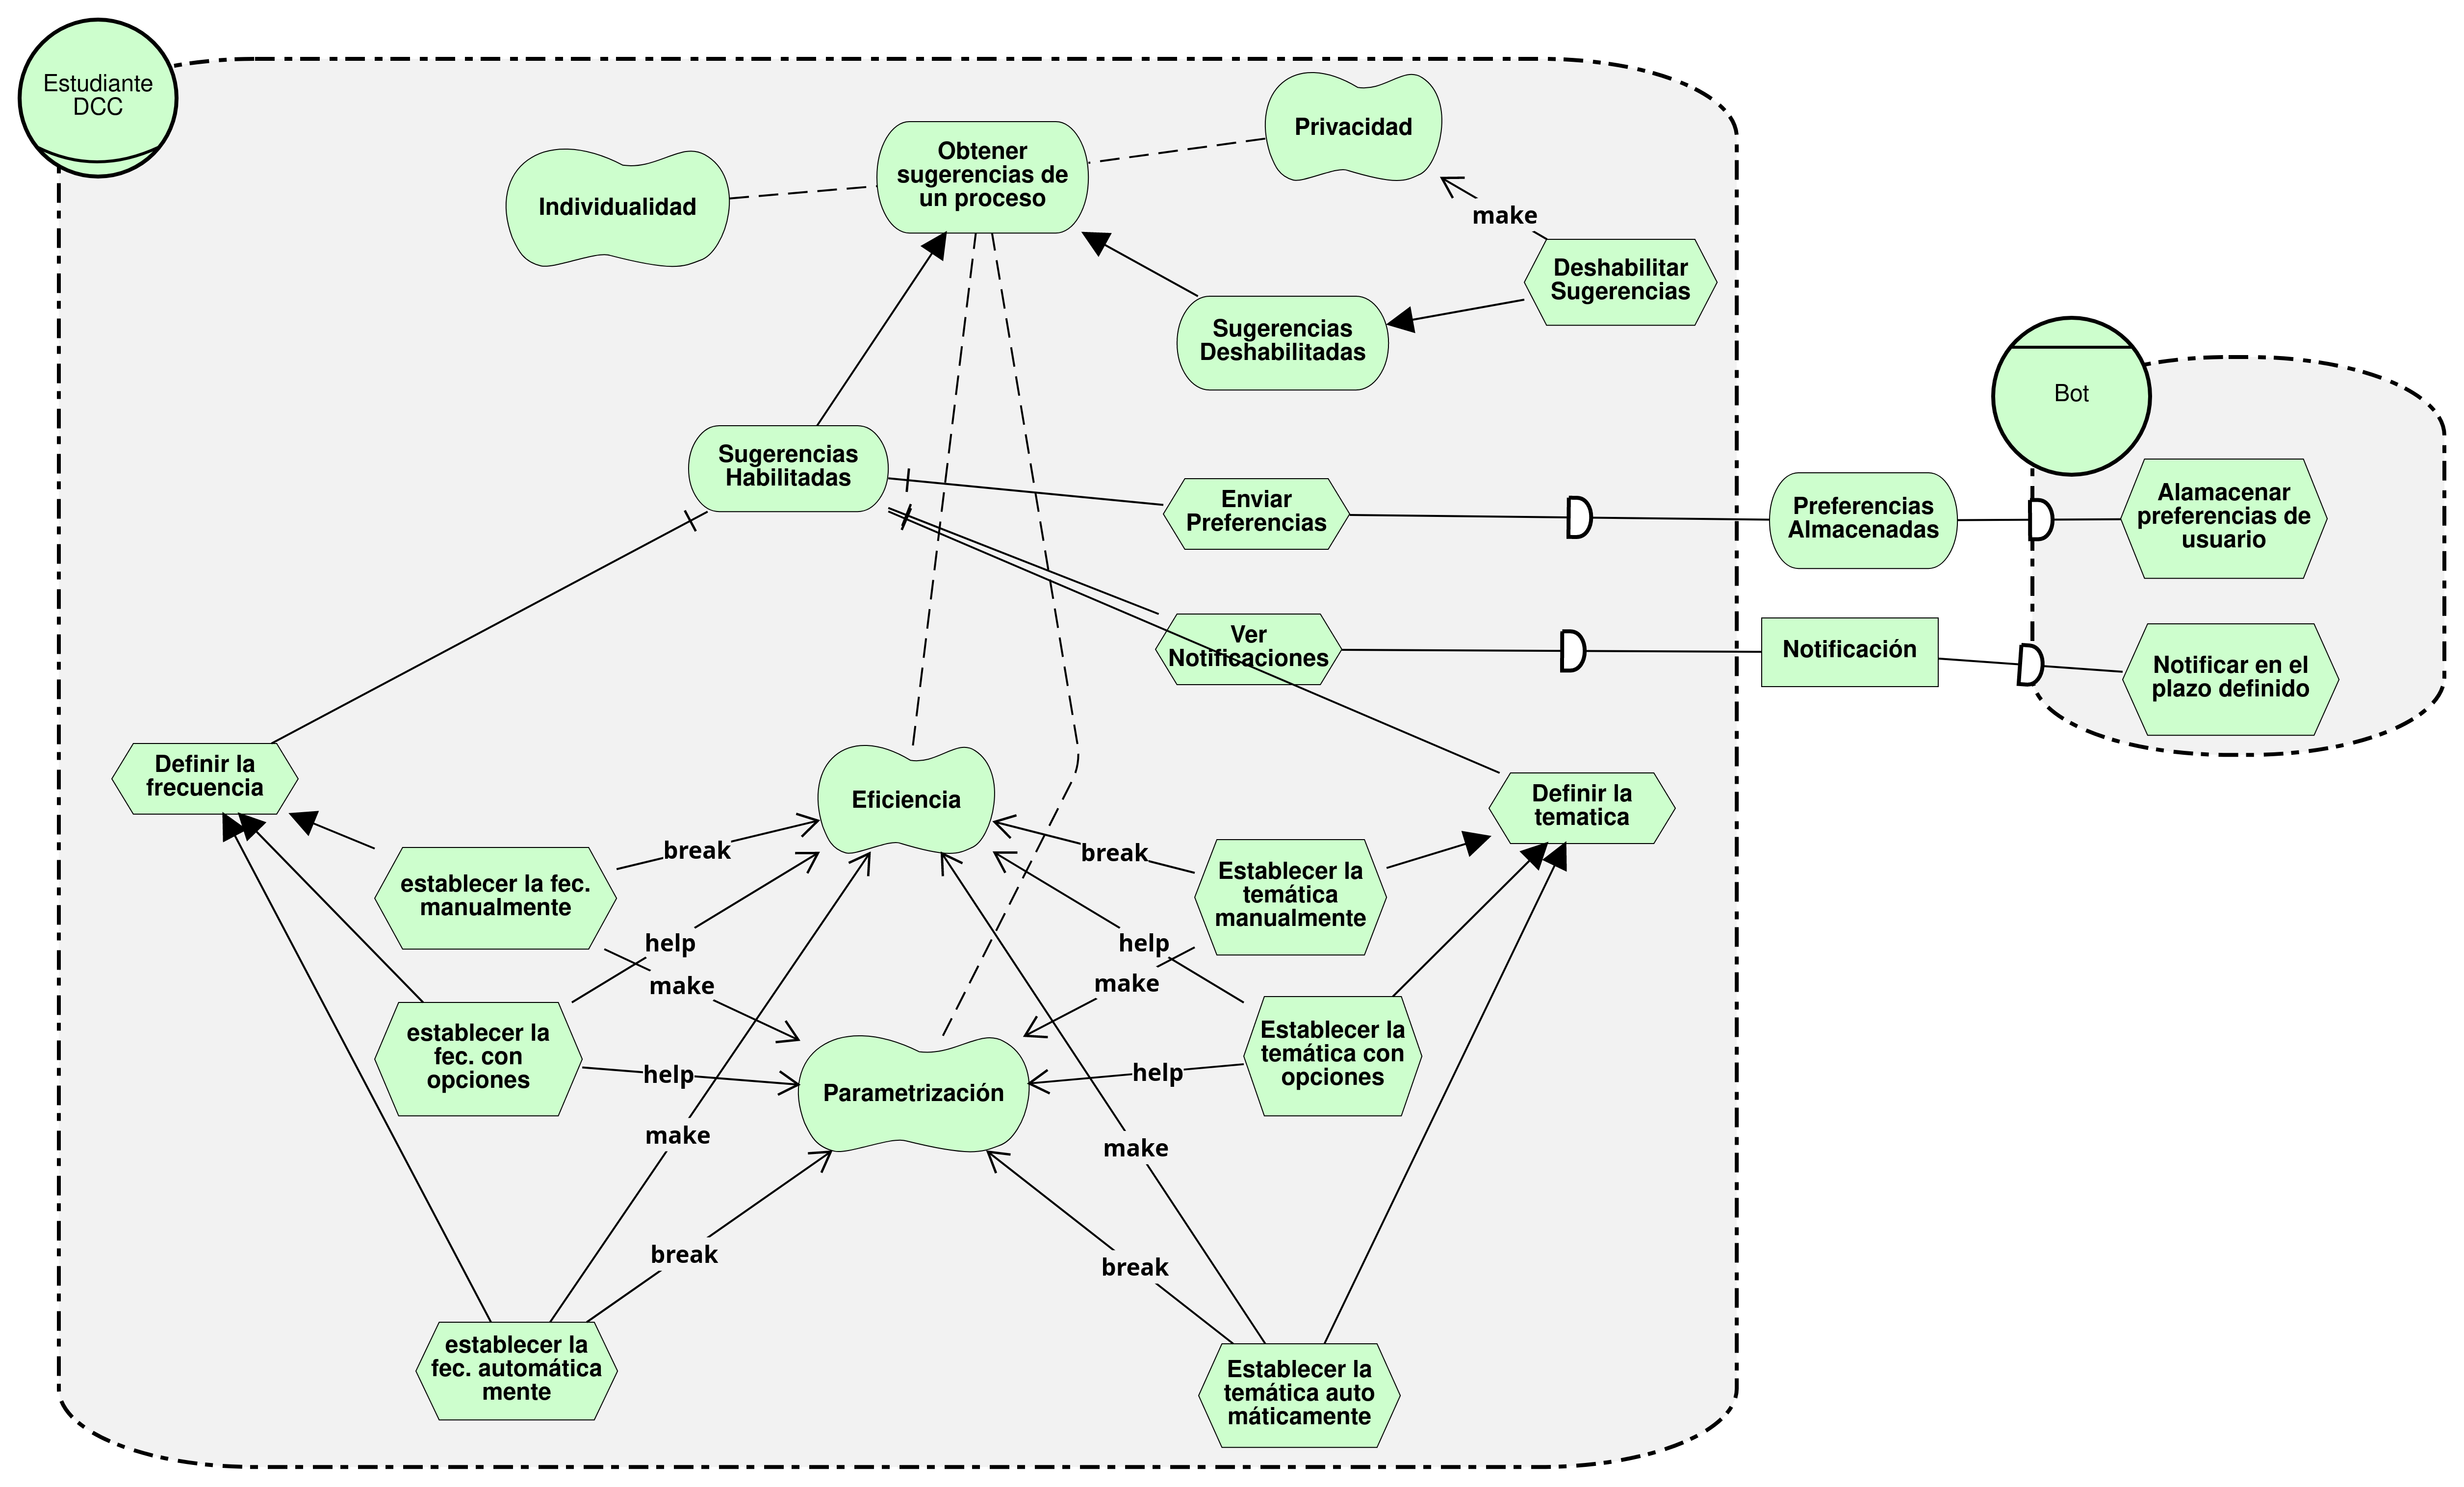
\includegraphics[width=\textwidth]{02-informe/imagenes/modelos_de_interacción/Sugerencias.png}
        \caption{Este diagrama representa un modelo de Interacción para la obtención de sugerencias a través del bot, sobre temas relacionados con las suscripciones de un usuario, siendo estas relativas a un proceso. En sintaxis i* 2.0}
        \label{fig:sugerencias}
    \end{figure}
    
    \par Las sugerencias son una de las interacciones más complicadas a nivel cualitativo lo que posteriormente puede tener un impacto en el desarrollo. Sin embargo, dependiendo del grupo de alumnos, puede ser una cualidad muy deseada como algo totalmente opuesto a las preferencias. Por dicha razón, la validación posterior al desarrollo debe ser cuidadosa, ya que si no se muestrea de manera representativa se podría sesgar el resultado y cargarlo para un sector, lo que podría hacer que ciertas modalidades parecieran irrelevantes para desarrollos posteriores.
    \par Al igual que los recordatorios deben ser establecidas en plazos. Por otro lado, se deben definir temáticas sobre las cuales entregar sugerencias al estudiante. Esto abre un abanico bastante amplio sobre el cual determinar estas temáticas, y cuando es útil una modalidad sobre la otra. Porque si bien es evidente que un \acrshort{S} preferiría cierta modalidad para establecer la frecuencia, no es tan evidente si su tendencia a la privacidad los excluiría por completo de querer sugerencias. Por otro lado, algo que no se puede extrapolar del diagrama es que un \acrshort{P}, posiblemente ni siquiera solicitaría las sugerencias a pesar de desearlas.
    
    \newpage
    \textbf{Intervenciones}
    \begin{figure}[h!]
        \centering
        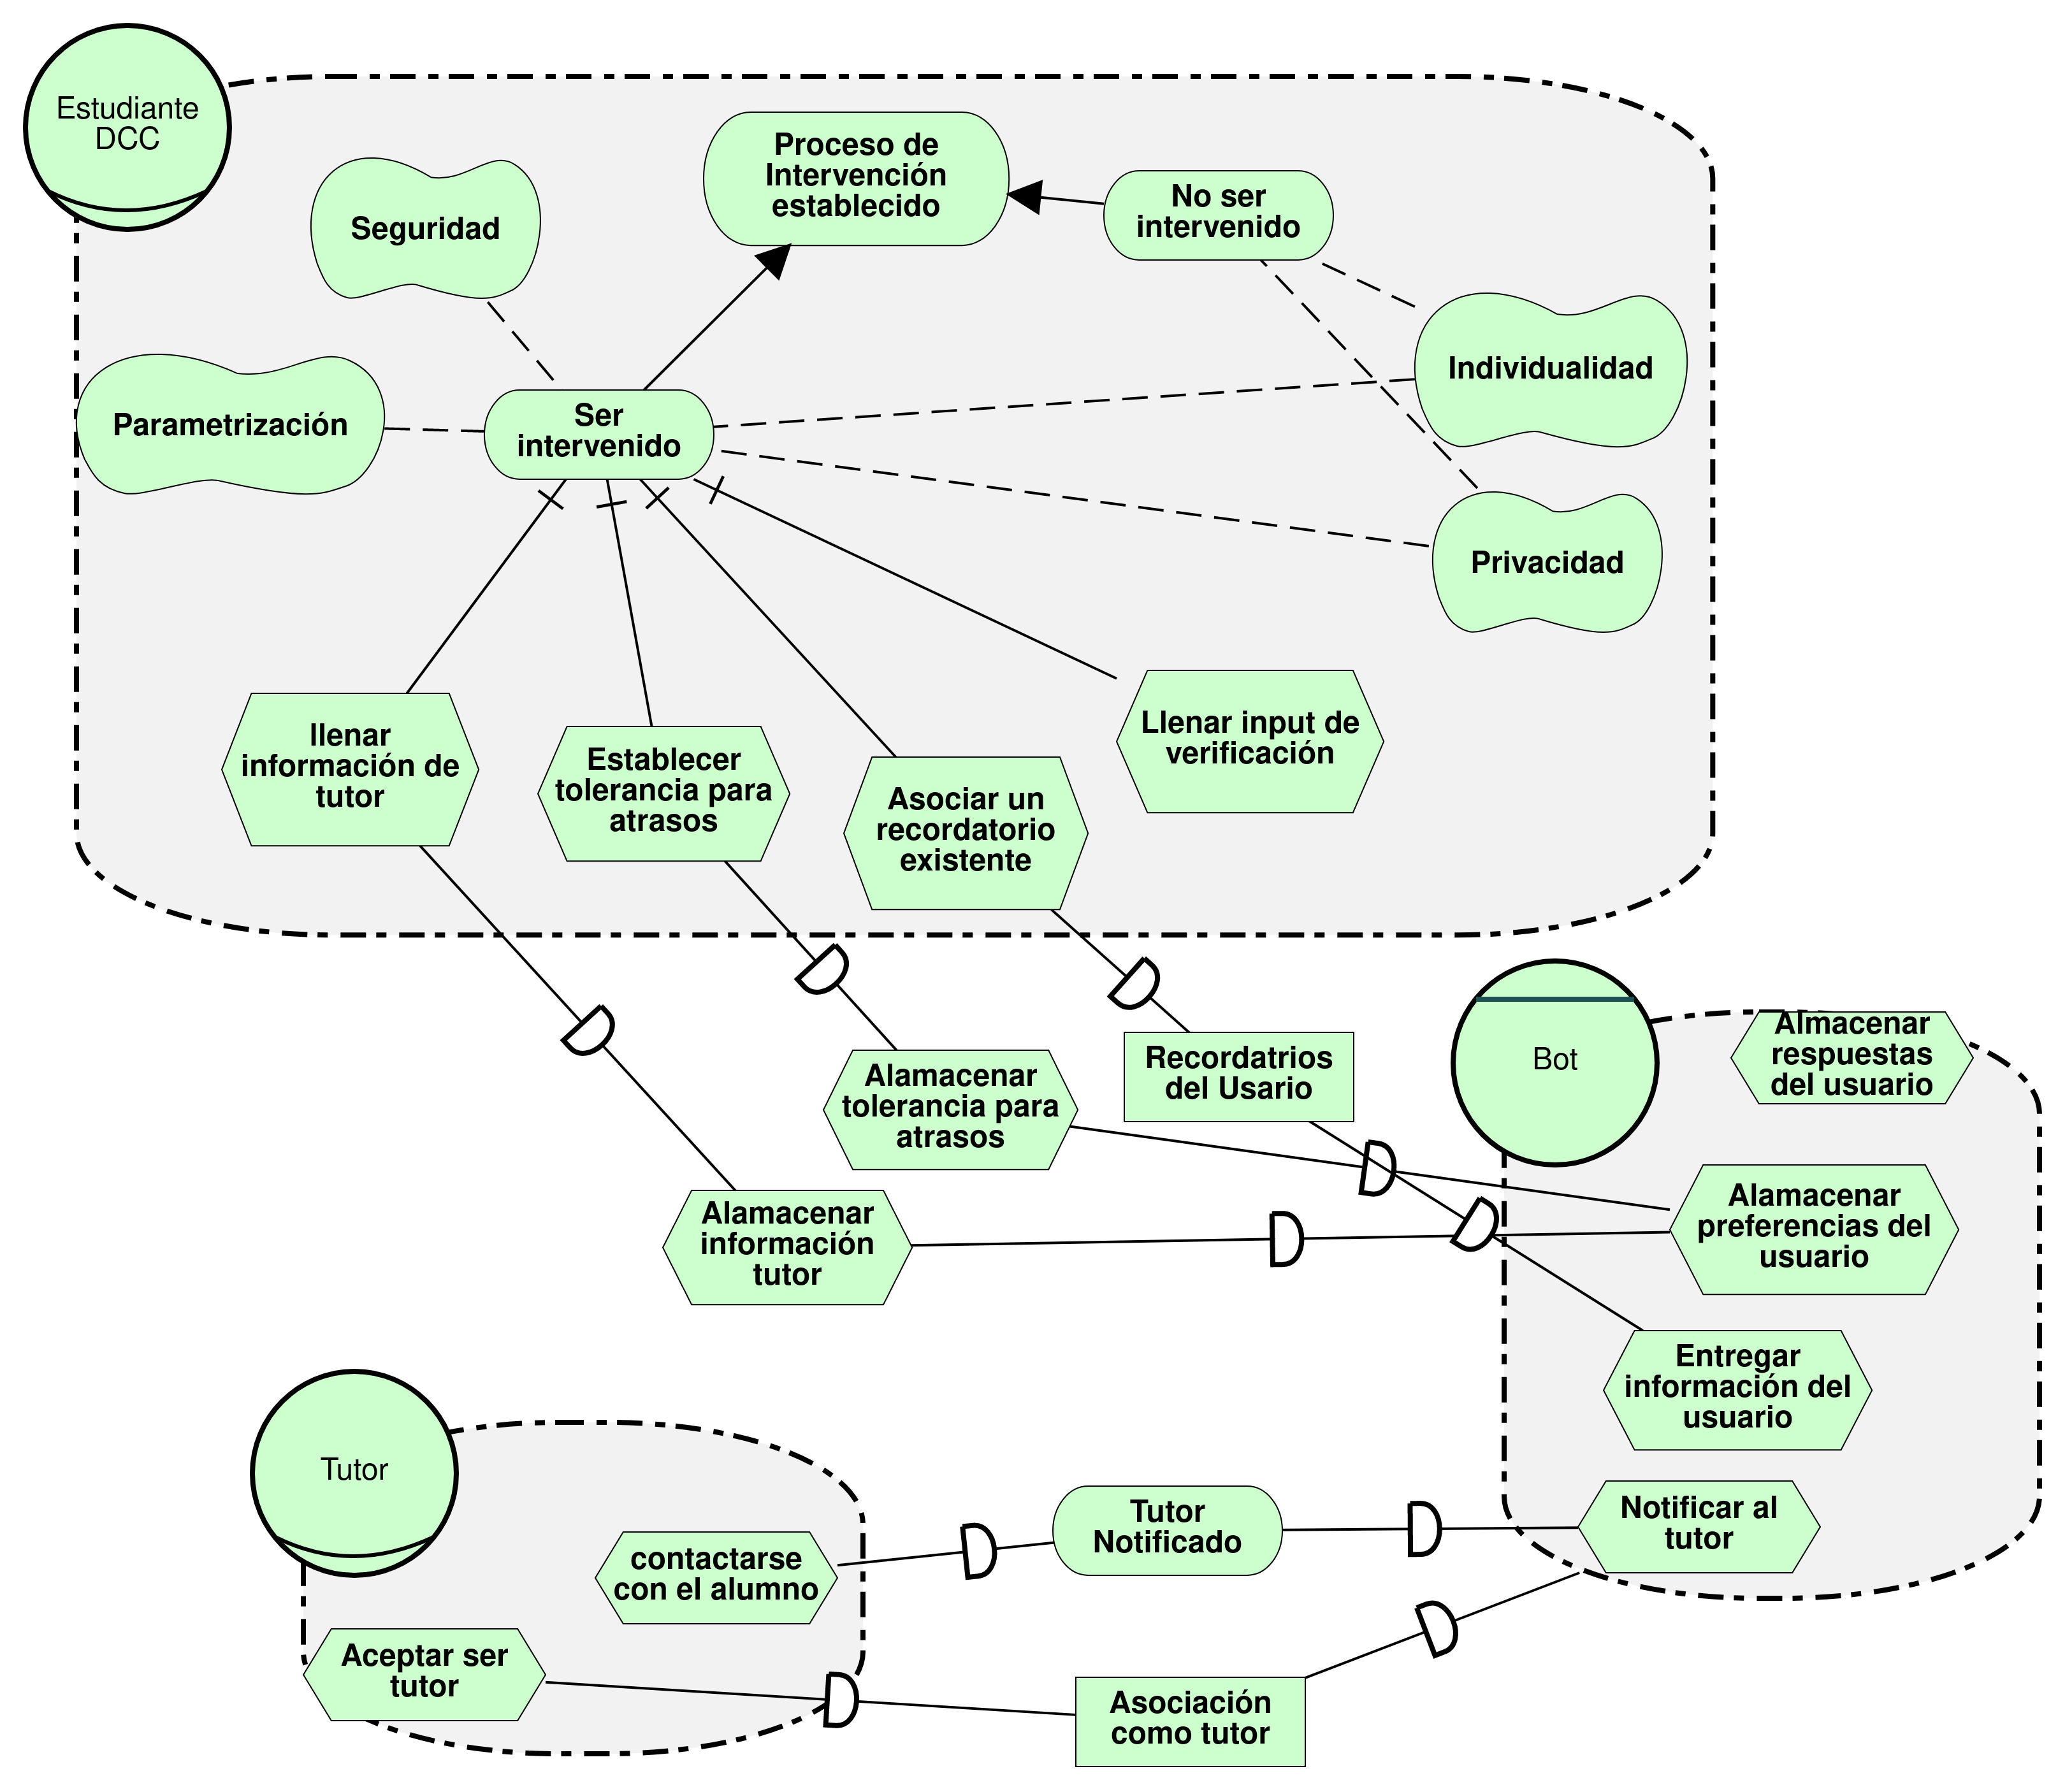
\includegraphics[width=\textwidth]{02-informe/imagenes/modelos_de_interacción/Intervenciones.png}
        \caption{Modelo de Interacción del proceso de intervención relativa a un proceso en el bot. En sintaxis i* 2.0}
        \label{fig:intervenciones}
    \end{figure}
    
    \par Las interacciones son las únicas funcionalidades que necesariamente involucran un tercero, el cual depende completamente del bot para determinar el momento cuando actuar.
    Esto hace que la configuración del alumno tome especial relevancia, y en ese sentido se puede ver que hay varias cualidades relacionadas con este objetivo.
    \par otra de las observaciones relevantes es que se necesita un consentimiento del tutor para ejercer tales funciones, y que estas están fuera del alcance del sistema. Así mismo, la interacción usuario bot se hace muy relevante, esto hace que se entre una paradoja de difícil resolución, un \acrshort{S} probablemente descartaría toda la funcionalidad de plano, y aunque un \acrshort{P} probablemente quiera este tipo de funcionalidad la interacción posterior a la configuración inicial puede desalentarlo de llevarlo a cabo por completo.
    
    \subsection{Conclusión y próximos pasos}
    \par A pesar de ser un modelo cualitativamente complejo, gracias a la modelación por i* se pudieron simplificar las interacciones sin dejar de dar cuenta de las diferentes opciones de cada uno de los alumnos en el sistema. Esto se traduce en que la personalización uno de los objetivos fundamentales del sistema se puede traducir en elementos puramente funcionales, lo que permitiría que responderían a un mismo módulo de programación en el futuro. Por ejemplo, las sugerencias son deseadas o no por los diferentes tipos de alumnos por lo cual se deben habilitar, esto responde a elementos de privacidad e individualidad, una vez habilitadas, el sistema se podría hacer cargo de todo de manera completamente invisible para el alumno, como podrían ser parametrizadas por completo lo que responde a las cualidades de parametrización y eficiencia deseadas por los usuarios.
    \par Un aspecto digno de otro estudio encontrado durante esta investigación es que los alumnos desean tanto elementos que faciliten alguna tarea específica  ligada al proceso como funcionalidades de carácter más educativo que buscan expresar de manera más clara y simple, pero al mismo tiempo, de forma posiblemente más reiterativa de que consiste el proceso.
    \par Este fenómeno da cuenta de que para el ingreso y paso exitoso de un alumno por un proceso académico no es suficiente con tener la información disponible o tener vías de consulta de dudas, sino que se debe formar al alumno en el proceso, al mismo tiempo que se debe acompañar durante el mismo. Esto necesariamente implica que los aspectos docentes y tutoriales presentes en los cursos regulares son de alguna manera necesarios para estos procesos académicos.
    \par Sin embargo estos análisis y la búsqueda de posibles causas se escapa de los alcances de esta memoria.
    \par Dentro de lo inmediatamente siguiente, estaría traducir los modelos de interacción a modelos de un carácter más funcional, esto se planea hacer a través de un modelamiento con UML, al mismo tiempo hay que realizar nuevos modelos de datos que puedan dar cuenta de las nuevas características necesarias en un proceso.
    \par Finalizado este diseño, se pasaría a implementar las nuevas funcionalidades en el sistema.
